\pagebreak
\section{Explosi\'on del transbordador espacial Challenger: un an\'alisis estad\'istico del accidente del Challenger}


Una comprensi\'on profunda del desastre requiere un an\'alisis estad\'istico de
los datos disponibles de las juntas t\'oricas que contienen informaci\'on sobre
la temperatura y las tasas de \'exito/fallo. Analizar las fallas de las juntas
t\'oricas requiere una comprensi\'on de la estructura subyacente de Challenger.
Los propulsores de cohetes del transbordador ten\'ian cuatro segmentos. 

\begin{wrapfigure}{r}{0.5\textwidth} \vspace{-20pt} 
    \begin{center}
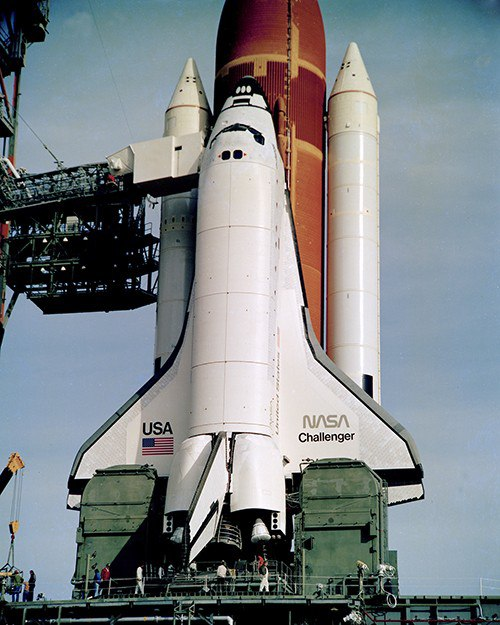
\includegraphics[width=0.48\textwidth]{figures/challenger.jpg} \end{center}
\vspace{-20pt} \caption{Challenger} \vspace{-10pt} \end{wrapfigure} 

En primer lugar, lleno de combustible. En segundo lugar, oxidante. Y la NASA los
ensambl\'o y sell\'o con juntas t\'oricas, un componente cr\'itico que evit\'o
la fuga de gas caliente durante el lanzamiento.Sin embargo, la capacidad de
respuesta de los sellos no se prob\'o en temperaturas fr\'ias. \\


El d\'ia del lanzamiento, la temperatura era de 31 grados Fahrenheit,
significativamente m\'as baja que las temperaturas en las que se probaron las
juntas t\'oricas. Despu\'es del despegue, una de las juntas t\'oricas se
rompi\'o, lo que provoc\'o que el gas caliente calentara el ox\'igeno l\'iquido
y el hidr\'ogeno dentro de los tanques. finalmente rompiendo los propulsores y
destrozando el transbordador 1 . Entonces, ¿por qu\'e se tom\'o la decisi\'on de
continuar con el lanzamiento, a pesar de las advertencias de los ingenieros? \\


Antes del lanzamiento del Challenger, nadie hab\'ia analizado la asociaci\'on
entre la temperatura y la capacidad de respuesta de las juntas t\'oricas. La
NASA decidi\'o arriesgarse al lanzar el transbordador, sin conocer la verdadera
probabilidad estad\'istica de fallas en las juntas t\'oricas a 31 grados. \\ 

Las preocupaciones de los ingenieros se basaban en sospechas y an\'alisis
incompletos. Los ingenieros solo observaron los datos de las juntas t\'oricas de
baja temperatura que inclu\'ian 4 fallas. Al ignorar los datos sobre vuelos a
temperaturas m\'as altas, la probabilidad de falla calculada fue menor de lo que
deber\'ia haber sido 2 . Este an\'alisis no solo es incorrecto sino tambi\'en
peligroso y condujo al desastre. \\

Se deben tener en cuenta los datos de todos los vuelos que se registraron. Ha
habido muchas fallas de juntas t\'oricas tanto a altas como a bajas
temperaturas, pero no se ha medido la fuerza de la asociaci\'on entre estas dos
variables. Los ingenieros no pueden simplemente ignorar los vuelos con
temperaturas m\'as altas.\\

Se requiere un an\'alisis estad\'istico profundo de la eficiencia de las juntas
t\'oricas a varias temperaturas para comprender realmente la falla del
Challenger. Las intuiciones y los an\'alisis sesgados, especialmente por parte
de la administraci\'on de la NASA, no son suficientes para determinar la
probabilidad de falla de las juntas t\'oricas.\\

A continuaci\'on se muestra una muestra de los datos de fallas de las juntas
t\'oricas:\\


\begin{landscape} 


\begin{table}[h]
\caption{Muestra de datos de O-Rings}
\begin{turn}{0}

\centering

\begin{tabular}{|l|l|l|l|} 
\hline
Vuelo & Fecha    & N\'umero de fallas de O-Ring primarias en juntas de campo & Temperatura de junta  \\ 
\hline
1     & 4/12/81  & 0                                                               & 66                    \\
2     & 11/12/81 & 1                                                               & 70                    \\
3     & 3/22/82  & 0                                                               & 69                    \\

5     & 11/11/82 & 0                                                               & 68                    \\
6     & 4/04/83  & 0                                                               & 67                    \\
7     & 6/18/83  & 0                                                               & 72                    \\
8     & 8/30/83  & 0                                                               & 73                    \\
9     & 11/28/83 & 0                                                               & 70                    \\
41-B  & 2/03/84  & 1                                                               & 57                    \\
41-C  & 4/06/84  & 1                                                               & 63                    \\
41-D  & 8/30/84  & 1                                                               & 70                    \\
41-G  & 10/05/84 & 0                                                               & 78                    \\
51-A  & 11/08/84 & 0                                                               & 67                    \\
51-C  & 1/24/85  & 2 (hubo otra, secundaria, falla en el O-Ring)                     & 53                    \\
51-D  & 4/12/85  & 0                                                               & 67                    \\
51-B  & 4/29/85  & 0                                                               & 75                    \\
51-G  & 6/17/85  & 0                                                               & 70                    \\
51-F  & 7/29/85  & 0                                                               & 81                    \\
51-I  & 8/27/85  & 0                                                               & 76                    \\
51-J  & 10/03/85 & 0                                                               & 79                    \\
61-A  & 10/30/85 & 2                                                               & 75                    \\
61-B  & 11/26/85 & 0                                                               & 76                    \\
61-C  & 1/12/86  & 1                                                               & 58                    \\
\hline
\end{tabular}
\end{turn}
\end{table}

\end{landscape} 

Se puede ejecutar una prueba de permutaci\'on para evaluar la importancia
estad\'istica de la diferencia entre la tasa de falla de la junta t\'orica a
bajas temperaturas y la tasa de falla a altas temperaturas. Esto puede
determinar si las juntas t\'oricas de temperatura m\'as baja tienden a
experimentar m\'as fallas que las juntas t\'oricas de temperatura alta, o si la
distribuci\'on de fallas es la misma entre las dos. Las hip\'otesis de esta
prueba estad\'istica son las siguientes:\\

\begin{equation} 
    H_o: Falla_{bajaTemperatura} - Falla_{altaTemperatura} = 0
\end{equation} 

La verdadera diferencia media entre la tasa de falla de la junta t\'orica a baja
y alta temperatura es 0. Las diferencias observadas se deben al azar.


\begin{equation}   
    H_o: Falla_{bajaTemperatura} - Falla_{altaTemperatura} > 0
\end{equation} 


La verdadera diferencia media entre la tasa de falla de la junta t\'orica a baja
y alta temperatura es mayor que 0. Las diferencias observadas no se deben al
azar, sino a una asociaci\'on entre la temperatura y la tasa de falla.\\

La permutaci\'on se ejecuta agrupando cada punto de datos en dos grupos. Alta y
baja temperatura. Mirando la distribuci\'on de temperatura. Las observaciones de
juntas t\'oricas se pueden dividir en menos de 65 grados (baja temperatura). Y
por encima de 65 grados (alta temperatura).\\

La diferencia media observada de fallos entre juntas t\'oricas de baja y alta
temperatura es de 1,3; la columna de temperatura se permuta (baraja). Y la
diferencia de falla media simulada la calculamos nuevamente entre los dos grupos
de juntas t\'oricas. La ejecuci\'on de 10 000 simulaciones de esta prueba de
permutaci\'on produce 10 000 estad\'isticas de prueba simuladas. A partir de
esto, podemos calcular el valor p para evaluar la hip\'otesis nula:

\begin{equation} \label{eq1}
    \begin{split}
\frac{sum(diferencias\;simuladas> diferencia\;observada)}{total\; intentos})=\\ \\
= \frac{sum(diferencias \;simuladas>1.3)}{1000}= \\ \\
=0.012
    \end{split}
\end{equation}


Solo el $1,2 \%$ de las diferencias medias de fallas simuladas son mayores que
la diferencia media de fallas observada. Un valor p de 0.012 es
estad\'isticamente significativo para rechazar la hip\'otesis nula que establece
que las tasas de falla de las juntas t\'oricas en temperaturas bajas y altas
provienen de la misma distribuci\'on.\\

La diferencia observada es mucho mayor que las diferencias en los datos de las
juntas t\'oricas barajadas. Esto sugiere que la tasa de fallas entre las juntas
t\'oricas de baja y alta temperatura no tiene la misma distribuci\'on. \\Los
datos muestran evidencia que respalda la hip\'otesis alternativa que establece
que las juntas t\'oricas de baja temperatura tienen una mayor tasa media de
fallas que las juntas t\'oricas de alta temperatura.\\

Definitivamente parece haber una diferencia entre las juntas t\'oricas probadas
a bajas temperaturas. Y las juntas t\'oricas se probaron a altas temperaturas,
pero es \'util examinar el modelo subyacente de los datos.\\

Es importante estimar la probabilidad de falla de la junta t\'orica a una
temperatura determinada. Esto se puede hacer ajustando un modelo de regresi\'on
log\'istica a los datos anteriores. Con temperatura como entrada y un valor
binario (1: al menos una falla, 0: ninguna falla) como salida. Ajustamos una
regresi\'on log\'istica con los siguientes par\'ametros:

\begin{equation} 
    P(Falla)= \frac{1}{1+exp^{-(\beta_0+\beta_1*temperatura)}}
\end{equation} 


Cuando $\beta_0$ es el coeficiente de temperatura que mide la asociaci\'on y  
$\beta_0$ es el sesgo.Adem\'as, probamos la fuerza de la asociaci\'on calculando
un valor z con respecto a las siguientes hip\'otesis:


\begin{equation} 
H_0 : \beta_1 = 0
\end{equation} 

El verdadero coeficiente de temperatura para el modelo es 0, lo que indica que
no hay relaci\'on entre la temperatura y la falla de la junta t\'orica.

\begin{equation} 
H_0 : \beta_1 \not {0}
\end{equation} 

El verdadero coeficiente de temperatura para el modelo no es 0, lo que indica
alguna relaci\'on entre la temperatura y la falla de la junta t\'orica.\\

Ajustar los datos a una regresi\'on log\'istica genera un modelo con los
siguientes pesos:

\begin{equation} 
P(Falla)= \frac{1}{1+exp^{-(10.88+0.17*temperatura)}}
\end{equation} 

Una gr\'afica a continuaci\'on visualiza la distribuci\'on de fallas y el ajuste
del modelo:

\begin{center} 
    \begin{figure}[h]
    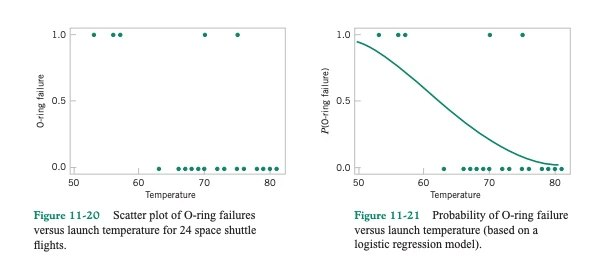
\includegraphics[width=12cm, height=9cm]{figures/challenger_plots.jpg}
    \caption{Gr\'aficas de regresi\'on log\'istica de datos de juntas te\'oricas.}
    \end{figure}
\end{center} 

Como se observa en la gr\'afica, una temperatura de 31 grados parece
incre\'iblemente probable que tenga al menos una falla. El modelo genera un
valor de 0,996, lo que indica un $99,6 \%$ de probabilidad de falla dados los
datos observados de lanzamientos de transbordadores anteriores.

Esto est\'a lejos de ser una decisi\'on cerrada y ciertamente no es una apuesta
arriesgada cuando hay siete compañeros de tripulaci\'on a bordo.

Adem\'as, la fuerza de la asociaci\'on entre estas dos variables. Analizamos con
el estad\'istico z generado en el peso del modelo del coeficiente de
temperatura. El valor p calculado de la hip\'otesis nula:


\begin{equation} 
H_0 : \beta_1 = 0
\end{equation} 


resulta ser 0,04, que es estad\'isticamente significativo cuando se utiliza un
umbral de 0,05. Debido al bajo valor de p, rechazamos la hip\'otesis nula que
establece que el coeficiente de temperatura es 0. Existe una fuerte evidencia en
los datos que respalda la hip\'otesis alternativa:

\begin{equation}  
H_0 : \beta_1 > 0
\end{equation} 


lo que sugiere que el coeficiente es mayor que 0 y que, de hecho, existe una
asociaci\'on entre la temperatura y la falla de la junta t\'orica. Por lo tanto,
existe una fuerte evidencia de que las bajas temperaturas pueden provocar fallas
en las juntas t\'oricas. Adem\'as, los ingenieros deber\'ian haber presentado un
an\'alisis de regresi\'on log\'istica como evidencia para retrasar el
lanzamiento del Challenger.\\

El desastre del Challenger muestra por qu\'e los cient\'ificos e ingenieros
necesitan comprender las t\'ecnicas estad\'isticas. Los an\'alisis b\'asicos
descritos brindan una s\'olida evidencia cuantitativa de que el transbordador no
deber\'ia haberse lanzado debido a la probabilidad significativamente alta de
falla de la junta t\'orica, un componente cr\'itico de la nave espacial.\\

